\documentclass[notes=show,9pt]{beamer}

\usepackage[english,russian,ukrainian]{babel}
\usepackage[cp1251]{inputenc}       % allow Latin1 characters

\usepackage{textcomp}
\usepackage{pgf}%,pgfarrows,pgfnodes,pgfautomata,pgfheaps

\usepackage{beamerthemeshadow}
\useinnertheme[shadow=true]{rounded}
%\usecolortheme[named=CarnationPink]{structure}
\usecolortheme{seahorse}
%\usecolortheme{whale}
\useoutertheme{shadow}
\usefonttheme{structureitalicserif}
%\usefonttheme[onlysmall]{structurebold}

\setbeamercolor{title}{use=structure,fg=white,bg=structure.fg}
\setbeamerfont{block title}{size={}}


\usepackage{times}

\usepackage{color}

\newcommand{\tblue}[1]{\textcolor{blue}{#1}}
\newcommand{\tred}[1]{\textcolor{red}{#1}}
\newcommand{\tgreen}[1]{\textcolor{green}{#1}}
\newcommand{\tyellow}[1]{\textcolor{yellow}{#1}}
\newcommand{\tbrown}[1]{\textcolor{brown}{#1}}
\newcommand{\tcyan}[1]{\textcolor{cyan}{#1}}
\newcommand{\tmagenta}[1]{\textcolor{magenta}{#1}}
\newcommand{\torange}[1]{\textcolor{orange}{#1}}
\newcommand{\tviolet}[1]{\textcolor{violet}{#1}}
\newcommand{\tpurple}[1]{\textcolor{purple}{#1}}

\newcommand{\tpink}[1]{\textcolor{pink}{#1}}
\newcommand{\tolive}[1]{\textcolor{olive}{#1}}
\newcommand{\tdarkgray}[1]{\textcolor{darkgray}{#1}}
\newcommand{\tgray}[1]{\textcolor{gray}{#1}}
\newcommand{\tlightgray}[1]{\textcolor{lightgray}{#1}}
\newcommand{\twhite}[1]{\textcolor{white}{#1}}

%\newcommand{\proclim}[2]{{\bf\sffamily #1} {\sffamily #2}}

\usepackage{verbatim}

\usepackage{graphicx}
\usepackage{amsmath,amssymb}

\usepackage{fancybox}

\usepackage{mathptmx}

\usepackage{lmodern}
\usepackage[T1]{fontenc}

\usepackage{mathpazo}

% \usepackage[sc]{mathpazo}
\usepackage{helvet}
\renewcommand{\familydefault}{\sfdefault}
\usepackage{pifont}

\usepackage{datetime}
\newdate{date}{28}{09}{2023}
\date{\displaydate{date}}


\beamertemplateshadingbackground{red!1}{blue!5}
\beamertemplatetransparentcovereddynamic
\beamertemplateballitem
\beamertemplatenumberedballsectiontoc
%\beamertemplatenotecompress

%\setbeamersize{sidebar width left=0.3cm,sidebar width right=0.3cm}
%{\usebeamercolor{yellow}}
%\setbeamertemplate{sidebar canvas left}[horizontal shading]
%[left=white,middle=yellow.bg,right=white]
%\setbeamertemplate{sidebar canvas right}[horizontal shading]
%[left=white,middle=yellow.bg,right=white]


 \DeclareMathOperator{\re}{Re}
 \DeclareMathOperator{\dist}{dist}
 \DeclareMathOperator{\ecc}{\overline{\mathrm{co}}}
 \DeclareMathOperator{\ec}{co}
\newcounter{equi1}
\newenvironment{equi}
{\begin{list}
        {$(\roman{equi1})$}
        {\setlength{\itemsep}{0ex plus 0.2ex minus 0ex}
         \setlength{\topsep}{0ex}
         \setlength{\parsep}{0ex}
         \setlength{\labelwidth}{7ex}
         \usecounter{equi1}}}
{\end{list}}

\renewcommand{\raggedright}{\leftskip=4pt \rightskip=4pt plus 0cm}

\hypersetup{pdfkeywords={pdftex, acrobat}, pdfpagemode={FullScreen}}



%\title[\twhite{\small \centerline{��� �������� ������� �� ����� �������������� �����}}]

\title[Using GitHub classroom for student education]{Using GiHub classroom for student education}


\author[Melnyk Vasyl]{\textbf{Melnyk Vasyl}}


\begin{document}


\begin{plainframe}
  \titlepage
\end{plainframe}



\begin{frame}{Git organisation used for student education}
\includegraphics[scale=0.4]{p_gitorg.PNG}
\end{frame}


\begin{frame}{Student evaluation}
\includegraphics[scale=0.3]{p_table.PNG}
\end{frame}


\begin{frame}{Githab classroom}
\includegraphics[scale=0.3]{p_classroom.PNG}
\end{frame}


\begin{frame}{Assignments in the classroom}
\includegraphics[scale=0.4]{p_classroom_labs.PNG}
\end{frame}


\begin{frame}{Create an assignment}
\includegraphics[scale=0.4]{p_assignment_creation.PNG}
\end{frame}


\begin{frame}{Autograding option}
\includegraphics[scale=0.4]{p_autograding.PNG}
\end{frame}


\begin{frame}{Test example}
\begin{center}
\includegraphics[scale=0.6]{p_test_example.PNG}
\end{center}
\end{frame}


\begin{frame}{Ready assignment}
\includegraphics[scale=0.4]{p_ready_assignment.PNG}
\end{frame}


\begin{frame}{Create template and yaml file with test check}
\includegraphics[scale=0.5]{p_yaml.PNG}
\end{frame}


\begin{frame}{Usage}
\begin{center}
\includegraphics[scale=0.45]{try_using.PNG}
\end{center}
\end{frame}


\begin{frame}{Completed assignment}
\includegraphics[scale=0.45]{p_assignment_completed.PNG}
\end{frame}


\begin{frame}{Autotests run}
\includegraphics[scale=0.6]{p_green_check}
\end{frame}


\begin{frame}{Github pages example}
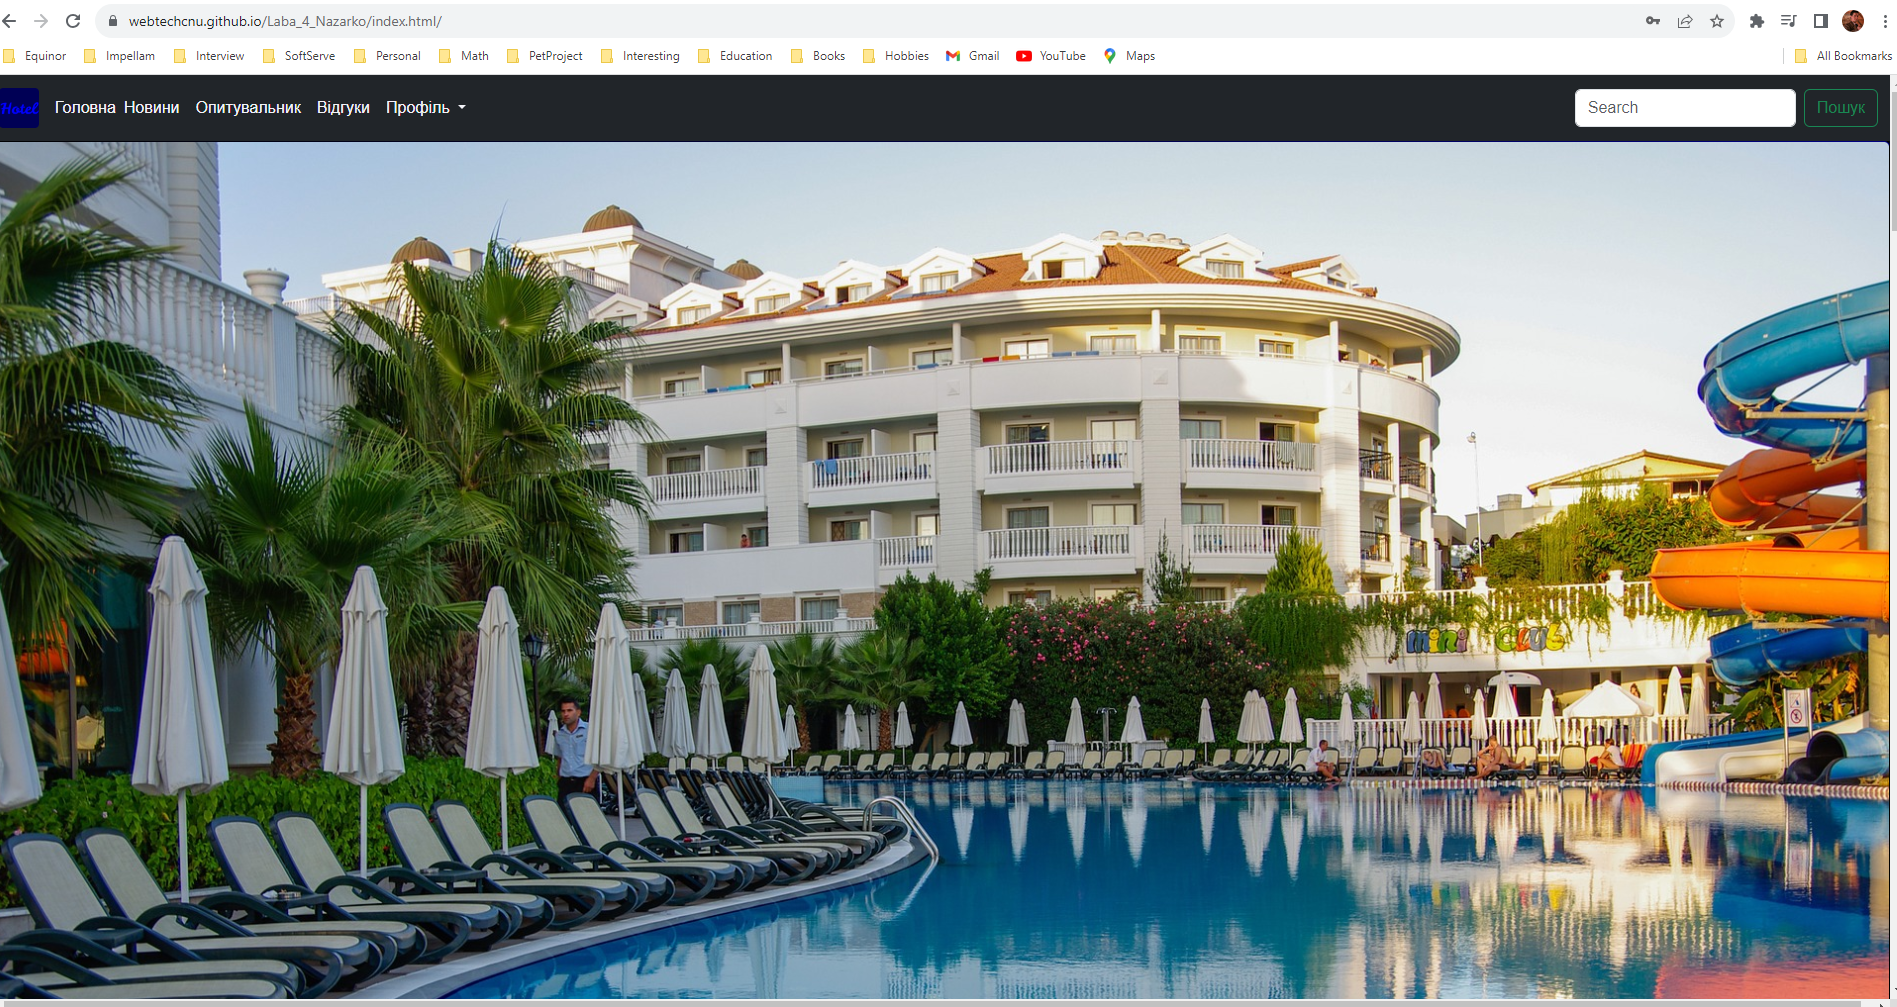
\includegraphics[scale=0.28]{p_git_page_exmpl.PNG}
\end{frame}


\begin{frame}{Github issues}
\includegraphics[scale=0.48]{p_github_issues.PNG}
\end{frame}


\begin{frame}{Github issues}
\includegraphics[scale=0.55]{p_issue_example.PNG}
\end{frame}




\begin{frame}\frametitle{}
\Huge \centerline{Thank you!}
\end{frame}

\end{document}

